% !TeX spellcheck = it_IT
\newpage
\subsection{Ebook reader}
Entro il 2025 si prevede che gli e-reader rappresenteranno circa il $75\%$ del mercato totale, anche se allo stesso tempo il numero di libri cartacei prodotti e  venduti è in continuo aumento.

\subsubsection{Ciclo di produzione}
Vediamo il ciclo di vita di un libro tradizionale cartaceo
\begin{center}
	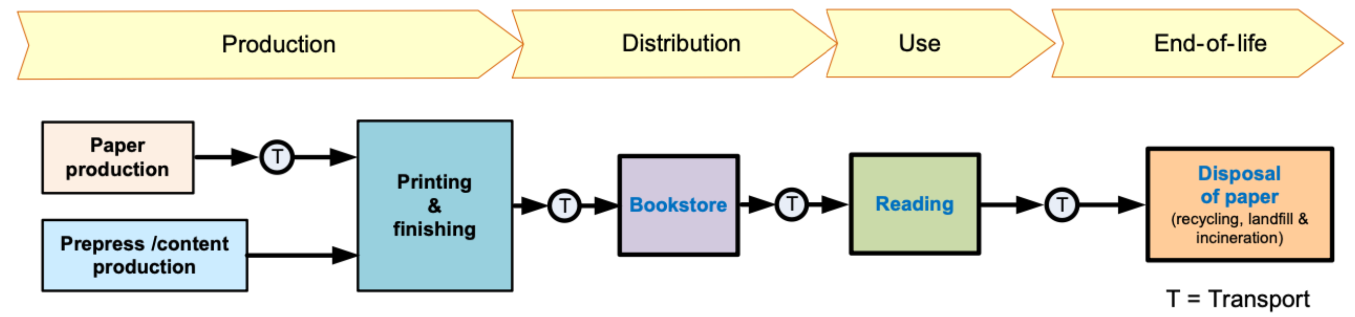
\includegraphics[scale=0.3]{books_lifecycle.png}
\end{center}
Le materie prime necessarie sono, per un libro a copertina morbida, $150-300$g di carta e $7.5$lt di acqua. Sono necessari $2$KWh  e la loro distribuzione (assumendo che non si usi la macchina per comprarlo) produce circa 10 volte quella della produzione. L'utilizzo è trascurabile dal punto di vista energetico in quanto al massimo serve una luce per leggere.
\begin{center}
	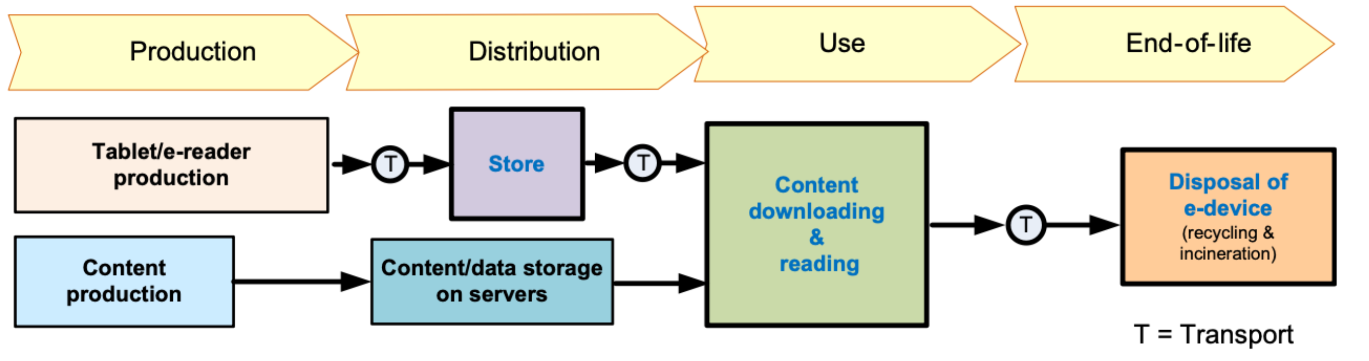
\includegraphics[scale=0.3]{ereader_lifecycle.png}
\end{center}
Per quanto riguarda invece gli e-book reader, sono necessari circa $15$Kg di materie prime (metalli rari, sabbia, etc...) e $300$lt di acqua (batterie, chip, oro dei circuiti). Sono necessari $100$KWh per la produzione e assumiamo i costi di distribuzione di un  \href{https://www.icao.int/environmental-protection/Carbonoffset/Pages/default.aspx}{\color{blue}volo Milano-Roma}.

\subsubsection{Confronto}
Considerando i dati precedenti:
\begin{enumerate}
	\item Quanti libri si producono con le materie prime necessarie per produrre un e-book reader?\\
	\begin{equation*}
		\frac{15Kg}{0.150Kg} = 100 \quad \frac{15Kg}{0.300Kg}=50
	\end{equation*}
	\item Quanti libri si producono con l'acqua necessaria per produrre un e-book reader?\\
	\begin{equation*}
		\frac{300lt}{7.5lt} = 40
	\end{equation*}
	\item Quanti libri si producono con l'energia necessaria per produrre un e-book reader?\\
	\begin{equation*}
		\frac{100KWh}{2KWh} = 50
	\end{equation*}
	\item Quanti libri serve produrre e trasportare per inquinare quanto per la produzione e il trasporto di un e-book reader?\\
	\begin{equation*}
		\begin{split}
			&\text{Produzione e-book reader}=0.319\frac{g}{Kw/h} \cdot 100Kw/h = 31.9Kg \quad \text{Distribuzione e-book reader}=41.8 Kg \\
			&\text{Totale e-book reader}=31.9Kg + 41.8Kg = 73.7 Kg \\
			&\text{Produzione libro}=0.319 \frac{g}{Kw/h} \cdot 2Kw/h = 0.638Kg \quad  \text{Distribuzione libro}= 0.638Kg \cdot 10 = 6.380Kg\\
			&\text{Totale libro}=6,380Kg + 0.638 Kg = 7.018Kg \\
			& \text{\textbf{Libri per e-book reader}}=\frac{73.7Kg}{7.018Kg}=10.5
		\end{split}
	\end{equation*}
	\item Qual'è la media dei valori delle risposte precedenti (quanti libri vale un e-book reader)?
	\begin{equation*}
		\frac{\frac{100+50}{2} + 40 + 50 + 10.5}{5} = 43.9
	\end{equation*}
	\item Quanti libri bisogna leggere all'anno per ammortizzare un e-book reader su 5 anni di vita media?
	\begin{equation*}
		\frac{43.9}{5} = 8.8
	\end{equation*}
\end{enumerate}

\subsubsection{Salute}
La produzione di libri ed e-book reader produce ossidi di azoto e zolfo che entrano in profondità nei polmoni, peggiorando l'asma, causando la tosse cronica e aumentando il rischio di morte prematura. Un e-book reader produce $70$ volte questi prodotti rispetto che ad un libro cartaceo.

\subsubsection{Dismissione}
\begin{table}[h]
	\begin{tabular}{|c|c|}
		\hline
		Libro & E-book reader \\
		\hline
		\multirowcell{2}{La \textbf{decomposizione} può generare il doppio \\delle emissioni e degli impatti tossici sulle \\ falde acquifere rispetto alla sua intera produzione} & \multirowcell{2}{In caso di \textbf{smaltimento illegale} in uno \\ dei paesi in via di sviluppo, i lavoratori\\ (spesso bambini) saranno esposti all'impatto\\ tossico di alcune sostanze smantellate. }\\
		\hline
		\multirowcell{2}{Può essere prestato, regalato, donato \\ad una biblioteca oppure correttamente riciclato. }& \multirowcell{2}{Se correttamente riciclato, molti materiali \\si potranno recuperare o smaltire correttamente.}\\
		\hline
	\end{tabular}
\end{table}

\subsection{Blockchain}
Bitcoin nasce nel 2008 come prima tecnologia basata sulla blockchain.
\begin{definition}[Blockchain]
	Blockchain è un libro mastro distribuito in grado di registrare e validare transazioni in assenza di un’entità centrale (e.g. banca).
\end{definition}
In particolare una blockchain ha le seguenti caratteristiche:
\begin{itemize}
	\item \textbf{Distribuita}: tutti i nodi partecipanti ne conservano una copia per trasparenza
	\item \textbf{Immutabile}: i record nella catena non possono essere né modificati né cancellati
	\item \textbf{Marcata temporalmente}: ogni transazione ha un timestamp
	\item \textbf{Unanime}: tutti i nodi partecipanti devono riconoscere la validità delle transazioni
	\item \textbf{Anonima}: l’identità dei partecipanti non è rivelata
	\item \textbf{Sicura}: tutti i record vengono criptati individualmente
	\item \textbf{Programmabile} per mezzo di SmartContracts
\end{itemize}

\subsubsection{Proof of Work}
La blockchain si basa sul concetto per cui ogni blocco, composto dalla transazione e dal riferimento a quella precedente, possa essere aggiunto solo quando viene fornita una \textbf{proof of work} da parte dei minatori, che risolvono problemi difficili (e.g. scomposizione in fattori primi).\\
Quando viene richiesta una transazione si crea un blocco che viene distribuito a tutti i partecipanti.\\
La difficoltà della proof of work aumenta con l'aumentare delle capacità computazionali dei nodi che scrivono nella blockchain, in modo tale da equilibrare:
\begin{itemize}
	\item \textbf{Sicurezza}: ad esempio evitando attacchi di doppia-spesa, o aggiunta di blocchi falsi 
	\item \textbf{Velocità di esecuzione} delle transazioni (stabilita attorno ai 10 minuti)
\end{itemize}

\subsubsection{Hardaware}
La potenza hardware per Bitcoin si misura in \textbf{GigaHash} al secondo (un hash è un calcolo da risolvere). L'hardware necessario si è evoluto con il tempo:
\begin{itemize}
	\item 2008 - \textbf{CPU}, $0.01GH/s$ con un consumo di $2.5Wh/GH$
	\item 2009 - \textbf{GPU}, $0.2-2GH/s$
\end{itemize}

\subsubsection{Minatori}
Possiamo suddividere le categorie dei minatori in:
\begin{itemize}
	\item \textbf{Piccoli}, il $15\%$ del totale, con un consumo fino a $0.1MW$ per $0.9PH/s$
	\item \textbf{Medi}, il $19\%$ del totale, con un consumo tra $0.1MW$ e $1MW$ per $9PH/s$
	\item \textbf{Grandi}, il $66\%$ del totale, con un consumo maggiore di $1MW$ per oltre $9PH/s$
\end{itemize}
I minatori si dividono in \textbf{pool} dove condividono il potere di calcolo:
\begin{center}
	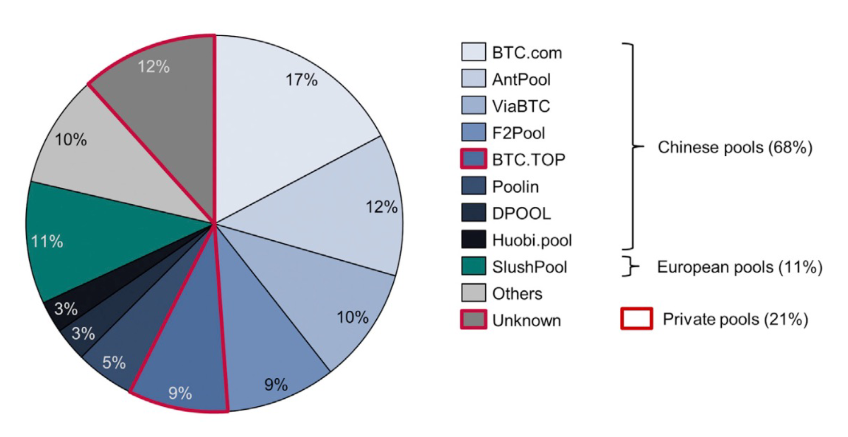
\includegraphics[scale=0.3]{bitcoin_pools.png}
\end{center}

\subsubsection{Analisi}
Consideriamo che al 2019 il consumo dell'hardware più efficiente era di $1.4 \cdot 10^{-5} Wh/GH$ e che per raffreddarlo veniva utilizzato il $5\%$ del consumo. Il numero di hash eseguiti in un'ora a novembre del 2019 era di $3.56 \cdot 10^{11} TH$. La localizzazione geografica dei minatori era:
\begin{itemize}
	\item \textbf{Cina} con il $68\%$ ad un costo di $0.55 \frac{kgCO_2-eq}{kWH}$
	\item \textbf{EU} con l'$11\%$ ad un costo di $0.28 \frac{kgCO_2-eq}{kWH}$
	\item \textbf{Privati} con il $21\%$ ad un costo di $0.475 \frac{kgCO_2-eq}{kWH}$
\end{itemize}
Considerando queste informazioni
\begin{enumerate}
	\item Qual è un limite inferiore al consumo energetico annuo di Bitcoin?
	\begin{equation*}
		\begin{split}
			&\text{Consumo per hash}=1.4 \cdot 10^{-5} \frac{Wh}{GH} + 5\% = 1.47 \cdot 10^{-5} \frac{Wh}{GH} \\
			&\text{Consumo per ora}=1.47 \cdot 10^{-5} \frac{Wh}{GH}  \cdot 3.56 \cdot 10^{14} GH = 5.2332 \cdot 10^9 W = 5.2332 \cdot 10^6 kW \\
			&\textbf{Consumo annuo}=5.2332 \cdot 10^6 kWh * 8760h = 4.5842832 \cdot 10^{10} kWh
		\end{split}
	\end{equation*}
	\item Quante emissioni di carbonio vengono prodotte all'anno se si utilizza quel limite inferiore come stima?
	\begin{equation*}
		\begin{split}
			&\text{Consumo \textbf{Cina}}=4.5842832 \cdot 10^{10} kWh \cdot 0.68 \cdot 0.55 \frac{kgCO_2-eq}{kWH} = 1.7145219168 \cdot 10^{10} kgCO_2-eq\\
			&\text{Consumo \textbf{EU}}=4.5842832 \cdot 10^{10} kWh \cdot 0.11 \cdot 0.28 \frac{kgCO_2-eq}{kWH} = 1.4119592256 \cdot 10^{9} kgCO_2-eq\\
			&\text{Consumo \textbf{privati}}=4.5842832 \cdot 10^{10} kWh \cdot 0.21 \cdot 0.475 \frac{kgCO_2-eq}{kWH} = 4.572822492 \cdot 10^{9} kgCO_2-eq
		\end{split}
	\end{equation*}
\end{enumerate}

\subsubsection{Oggi}
Nella primavera del 2021 alcuni stati come la Cina proibiscono il mining di Bitcoin e questo ha aumentato l'intensità del mining del $43\%$ rispetto al 2019. Si noti che al momento la Cabon Footprint del Bitcoin è di $77.42$ Mega Tonnellate di $CO_2$ ogni anno. In pratica una transazione con Bitcoin equivale a $1,000,000$ transazioni VISA.
\begin{center}
	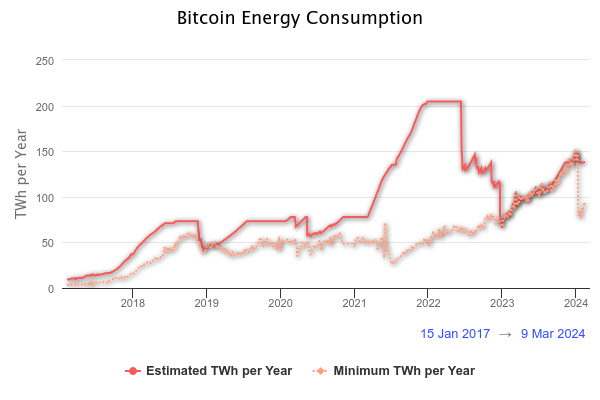
\includegraphics[scale=0.5]{bitcoin-energy-consumpti.png}
\end{center}
\begin{center}
	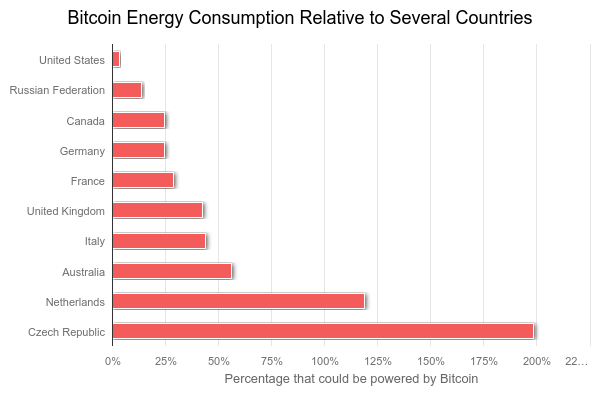
\includegraphics[scale=0.5]{bitcoin-energy-consumption_country.png}
\end{center}

Ad oggi esiste il \textbf{Crypto Climate Accord} che ha come obiettivo quello di contribuire a raggiungere gli Accordi di Parigi tramite l'utilizzo di energie rinnovabili entro il 2030.

\subsubsection{Conclusione}
La blockchain è una tecnologia all'avanguardia che potrebbe avere un impatto molto grande su molti settori. È importante eseguire un'analisi di costi e benefici per valutare se conviene o meno:
\begin{enumerate}
	\item \textbf{Emissioni} di carbonio
	\item Rischi di \textbf{centralizzazione}: se qualcuno ottenesse il $51\%$ della computing power avrebbe il controllo della blockchain
	\item Possibilità di \textbf{controllo} per evitare traffici illegali
\end{enumerate}

\subsubsection{Proof of Stake}
Per affrontare le problematiche indicate ai punti 1 e 2 si vorrebbe introdurre la \textbf{proof of stake}, dove l'abilità di minare è determinata in base alla quantità di moneta che un utente possiede. Il minatore non viene premiato con la moneta al completamento del calcolo ma con degli interessi. In questo modo si evita anche l'attacco del $51\%$ poiché si rende necessario avere il $51\%$ della moneta (più difficile).